\documentclass[9pt,twocolumn,twoside]{styles/osajnl}
\usepackage{fancyvrb}
\journal{i524} 

\title{Apache Flink: Stream and Batch Processing}


\author[1,*]{Jimmy Ardiansyah}

\affil[1]{School of Informatics and Computing, Bloomington, IN 47408, U.S.A.}


\affil[*]{jardians@indiana.edu - S17-IR-2002}

\dates{Research Article-02, \today}

\ociscodes{Apache Flink, Batch Data Processing, Stream Data Processing}

% replace this with your url in github/gitlab
\doi{\url{https://github.com/jardians/sp17-i524/blob/master/paper2/S17-IR-2002/report.pdf}}
 
\begin{abstract}
Apache Flink is an open-source system for processing streaming and batch data. Flink is built on the philosophy that many classes of data processing applications, including real-time analytics, continuous data pipelines, historic data processing (batch), and iterative algorithms can be expressed and executed as pipelined fault-tolerant dataflows. 
\newline  
\newline  
\end{abstract} 

   
\setboolean{displaycopyright}{true} 

\begin{document}

\maketitle

\section{Introduction}
Data stream  and batch data processing were traditionally considered as two very different types of applications. They were programmed using different programming models and APIs, and were executed by different systems. Normally, batch data analysis made up for the biggest share of the use cases, data sizes, and market, while streaming data analysis mostly served specialized applications. 

These continuous streams of data come for example from web log files, application log files, and databases log files. Rather than treating the streams as streams, today’s setups ignore the continuous and timely nature of data production. Instead, data records are batched into static data sets (hourly, daily, or monthly) and then processed in a time-based fashion. Data collection tools, workflow managers, and schedulers orchestrate the creation and processing of batches, in what is actually a continuous data processing pipeline. Apache Flink follows a paradigm that embraces data stream processing as the unifying model for real time analysis, continuous streams, and batch processing both in the programming model and in the execution engine. 

Flink programs can compute both data stream and batch data accurately that avoiding the need to combine different systems for the two use cases. Flink also supports different notions of time (event-time, ingestion-time, processing-time) in order to give programmers high flexibility in defining how events should be correlated. ~\cite{inproceeding-flink}. 

\section{History Development}
Flink has its origins in the Stratosphere project, a research project conducted by three Berlin-based Universities as well as other European Universities between 2010 and 2014. The project had already attracted a broader community base such as NoSQL and Big Data Developers Groups. This strong community base is one reason the project was appropriate for incubation under the Apache Software Foundation (ASF). 

A fork of the Stratosphere code was donated in April 2014 to the Apache Software Foundation (ASF) as an incubating project with an initial set of committers consisting of the core developer of the system. Shortly thereafter, many of the founding committers left university to start  a company to commercialize Flink such as Data Artisans.

During incubation, the project name had to be changed from Stratosphere because of potential confusion with an unrelated project. The name Flink was selected to honor the style of this stream and batch processor. In German, the word “Flink” means fast or agile. A logo showing a colorful squirrel was chosen because of squirrel are fast and agile. The project completed incubation quickly, and in December 2014, Flink graduated to become a top-level project of the Apache Software Foundation (ASF). Flink is one of the 5 largest big data projects of Apache Software Foundation (ASF) with a community of more than 200 developers across the globe and several production installations in Fortune Global 500 companies.  In Octorber2015, the Flink project held its first annual conference in Berlin called Flink Forward ~\cite{wiki-flink} ~\cite{book-flink}.

\section{Design}
The core computational fabric of Flink  (labeled as “Flink runtime” in the Figure-1) is a distributed system that accept streaming dataflow programs and executes them in a fault-tolerant manner in one or more machines. This runtime can run in a cluster as an application of YARN (Yet Another Resources Negotiator) or within a single machine which is very useful for debugging Flink applications.

The program accepted by the runtime are very powerful, but are verbose and difficult to program directly. For that reason, Flink offer developer-friendly APIs that layer on the top of the runtime and generate there streaming dataflow programs. Apache Flink includes two core APIs: a DataStream API for bounded or unbounded streams of data and a DataSet API for bounded data sets. Flink also offers a Table API, which is a SQL-like expression language for relational stream and batch processing that can be easily embedded in Flink’s DataStream and DataSet APIs. The highest-level language supported by Flink is SQL, which is semantically similar to the Table API and represents programs as SQL query expressions ~\cite{www-flink}.

\begin{figure}[H]
 \centering
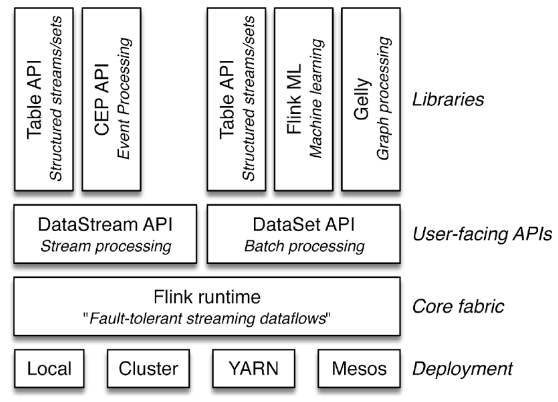
\includegraphics[scale=0.7]{images/image6}
\caption{Key concept of Flink Stack ~\cite{www-flink}}
\end{figure}

\subsection{Data Stream API}

DataStream programs in Flink are regular programs that implement transformations on data streams (e.g., filtering, updating state, defining windows, aggregating). The data streams are initially created from various sources (e.g., message queues, socket streams, files). Results are returned via sinks, which may for example write the data to files, or to standard output (for example the command line terminal). Flink programs run in a variety of contexts, standalone, or embedded in other programs. The execution can happen in a local JVM, or on clusters of many machines. The DataStream API includes more than 20 different types of transformations and is available in Java and Scala languages. A simple example of a stateful stream processing program is an application that emits a word count from a continuous input stream and groups the data in 5-second windows.

\begin{figure}[H]
 \centering
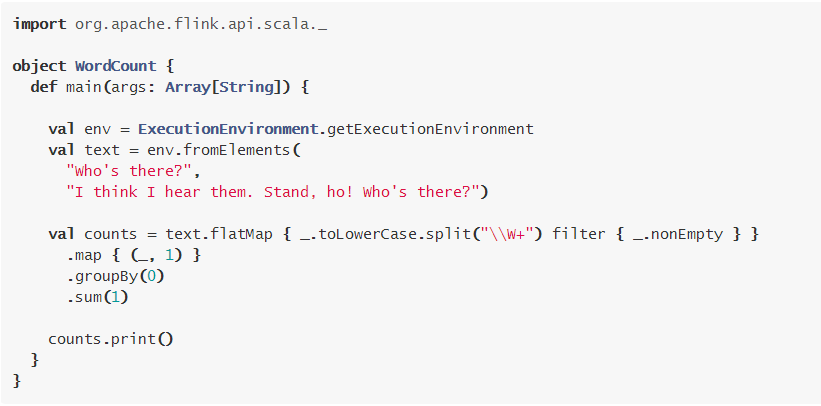
\includegraphics[scale=0.5]{images/image7}
\caption{Scala Example Program: Counts the words coming from a web socket in 5 second windows ~\cite{www-flink}}
\end{figure}

\subsection{DataSet API}

DataSet programs in Flink are regular programs that implement transformations on data sets (e.g., filtering, mapping, joining, grouping). The data sets are initially created from certain sources (e.g., by reading files, or from local collections).
Results are returned via sinks, which may for example write the data to (distributed) files, or to standard output (for example the command line terminal). Flink programs run in a variety of contexts, standalone, or embedded in other programs. The execution can happen in a local JVM, or on clusters of many machines.

\begin{figure}[H]
 \centering
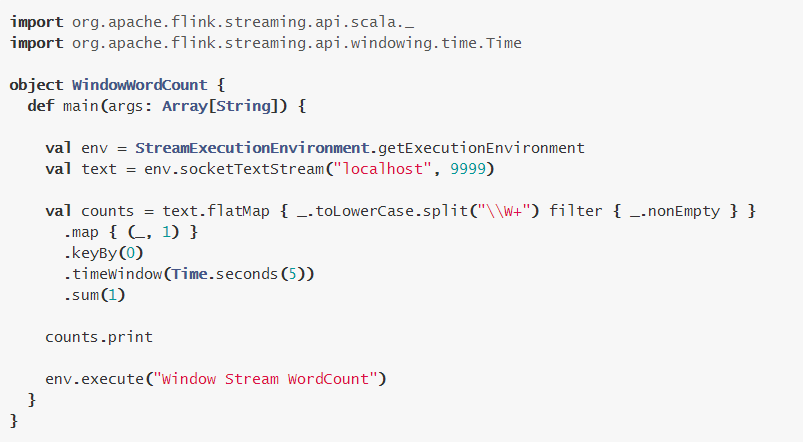
\includegraphics[scale=0.5]{images/image8}
\caption{Scala Example Program: WordCount  ~\cite{www-flink}}
\end{figure}

\subsection{ Table API}

The Table API is a declarative DSL centered around tables, which may be dynamically changing tables (when representing streams). The Table API follows the (extended) relational model: Tables have a schema attached (similar to tables in relational databases) and the API offers comparable operations, such as select, project, join, group-by, aggregate, etc. Table API programs declaratively define what logical operation should be done rather than specifying exactly how the code for the operation looks.

Though, the Table API is extensible by various types of user-defined functions, it is less expressive than the Core APIs, but more concise to use (less code to write). In addition, Table API programs also go through an optimizer that applies optimization rules before execution ~\cite{article-flink}. One can seamlessly convert between tables and DataStream/DataSet, allowing programs to mix Table API and with the DataStream and DataSet APIs. The highest level abstraction offered by Flink is SQL. This abstraction is similar to the Table API both in semantics and expressiveness, but represents programs as SQL query expressions. The SQL abstraction closely interacts with the Table API, and SQL queries can be executed over tables defined in the Table API.

\section{Implementation of Apache Flink }
\subsection{Alibaba}
~\cite{book-flink}This huge e-commerce group works with buyer and suppliers via its web portal. The company’s online recommendation are produced by Flink. One of the attractions of working with true streaming engines such as Flink is that purchases that are being made during the day can be taken into account when recommending products to users. This particularly important on special day (holidays) when the activities is unusually high. This is an example of a use case where efficient stream processing is a big advantage over batch processing.

\subsection{Otto Group}
~\cite{book-flink}The Otto is the world’s second-largest online retailer in fashion and lifestyle in Europe.  Otto had resorted to developing its own streaming engine because when it first evaluate the open source options, it could not find one that fit its requirement. After testing Flink, Otto found it fit their needs for streaming processing which include crowd-sourced user-agent identification, and a search session identifier.

\section{Conclusion}
Flink is not the only technology available to work with streaming and batch processing. There are a number of emerging technologies being developed and improved to address these needs. Obviously people choose to work with a particular technology for a variety of reason, but the strengths of Flink, the ease of working with it, and the wide range of ways it can be used to advantage make it an attractive option. That

\section{Acknowledgements}
This work was done as part of the course "I524: Big Data and Open Source Software Projects" at Indiana University during Spring 2017

% Bibliography

\bibliography{references}
 
\end{document}


